



\begin{frame}[t,allowframebreaks]{
    Momentum-based learning: Nesterov momentum -}

    \index{Nesterov momentum}\gls{Nesterov momentum} \cite{Nesterov:1983a}
    is a {\bf variant of the \index{momentum}\gls{momentum}}-based method.\\
    \vspace{0.2cm}
    In this algorithm, the update rule is given by:\\
    \vspace{-0.2cm}
    \begin{equation}
        \delta \vect{w}_{k} = 
          - \alpha \nabla_{\vect{w}} L(\vect{w}_{k}+\beta \delta \vect{w}_{k-1})
          + \beta \delta \vect{w}_{k-1}
        \label{eq:momentum_method_update_rule}
    \end{equation}
    \vspace{0.1cm}
    The only difference is that the \index{gradient}\gls{gradient}
    of the \index{loss function}\gls{loss function}, at step $k$, 
    is evaluated at $\vect{w}=\vect{w}_{k}+\beta \delta \vect{w}_{k-1}$
    rather than at $\vect{w}=\vect{w}_{k}$,
    \begin{itemize}
        \item i.e., the \gls{gradient} is 
        {\bf evaluated after adding the current \index{velocity}\gls{velocity}}.\\
    \end{itemize}

    \begin{center}
        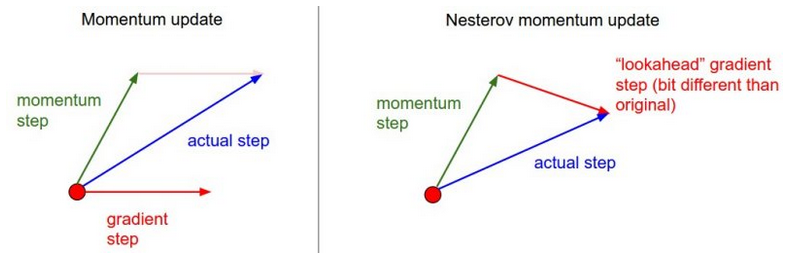
\includegraphics[width=0.80\textwidth]
            {./images/training_issues/cs231n_momentum_update_nesterov.png}\\
        {\tiny 
            \color{col:attribution} 
            Taken from \cite{CS231n}.\\    
        }
    \end{center}                

    \framebreak

    %
    %

    By {\bf looking ahead}
    (and evaluating the gradient after adding the \index{velocity}\gls{velocity}),
    \index{momentum}\index{Nesterov momentum}\gls{Nesterov momentum} 
    makes a correction to {\bf avoid overshooting}.\\

    \begin{center}
        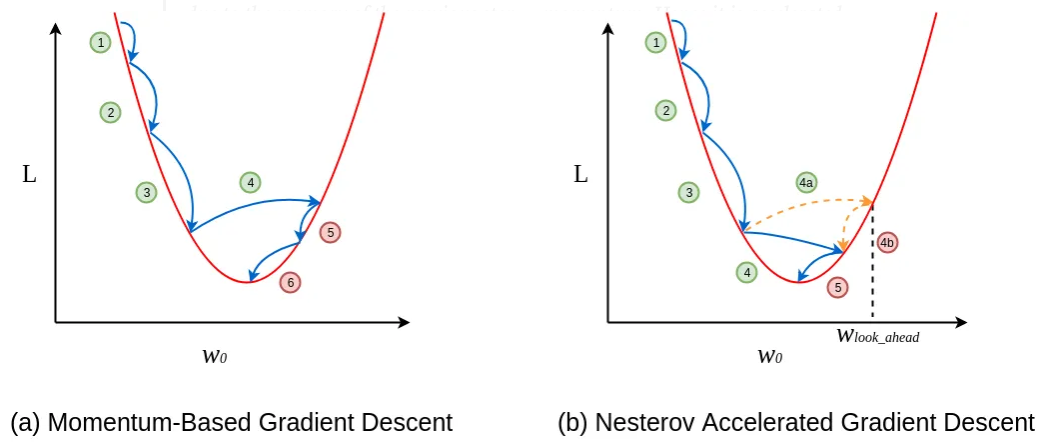
\includegraphics[width=0.88\textwidth]
            {./images/training_issues/chandra19_nesterov_momentum_updates.png}\\
        \vspace{0.1cm}
        {\scriptsize
            The plain \gls{momentum} method, based on reinforcement from previous 
            updates, takes a large step in update 4 and overshoots the minimum.
            It then recovers in steps 5 and 6.\\
            \gls{Nesterov momentum}, looks ahead before taking step 4, 
            and exploits that changing sign of the \index{gradient}\gls{gradient} 
             to try a smaller step.
            \color{col:attribution} 
            Taken from \cite{TowardsDataScience:LP2MomentumBasedGS}.\\    
        }
    \end{center}   
    
\end{frame}
